\documentclass[10pt]{article}

\usepackage[T1]{fontenc}
\usepackage[utf8]{inputenc}
\usepackage[margin=1in]{geometry}
\usepackage{amsmath}
\usepackage{amssymb}
\usepackage{newtxtext}
\usepackage{newtxmath}
\usepackage{microtype}
\usepackage{graphicx}
\usepackage{booktabs}
\usepackage{array}
\usepackage{tabularx}
\usepackage{rotating}
\usepackage{xurl}
\usepackage[numbers,sort&compress]{natbib}
\usepackage[colorlinks=true,linkcolor=blue,citecolor=blue,urlcolor=blue]{hyperref}
\usepackage{tikz}
\usetikzlibrary{arrows.meta,positioning}
\usepackage[fontset=fandol]{ctex}

\newcolumntype{Y}{>{\raggedright\arraybackslash}X}
\setlength{\tabcolsep}{4pt}

\title{Two Different Goals: Dissociating the Machine Mind from Artificial Intelligence}

\author{Yugui Yu\\ YYG Strategy Lab\\ \texttt{they4897@gmail.com}}

\date{November 5, 2026}

\begin{document}

\maketitle

\begin{abstract}
\noindent Public discourse, industry roadmaps, and parts of the academy read machine intelligence and machine mind as one road with milestones: the smarter the machine, the closer the heart. This paper defends the opposite as a matter of conceptual hygiene: artificial intelligence and the machine heart (机器之心; \emph{machine mind}) are two different goals, and the difference is teleological, not metaphysical. The first is an engineering goal---functional intelligence in the service of human practice---whose success criteria are public, dense, and continuously improving. The second is a realization goal---mind-structure genuinely instantiated, not merely simulated, in a non-biological substrate---imagined as achievable and pursued as science and engineering, yet still without a consensus third-person criterion. We make four contributions. (1)~A genealogy showing that the two goals formed and institutionalized independently: Turing's founding text bracketed consciousness while fixing a behavioral criterion; machine consciousness matured into a separate field with its own journals, workshops, societies, and moratoria, and a 2022--2026 dissociation wave has been gathering the same conclusion from theory-side, assessment-side, and relevance-side. (2)~A pathology of the binding in four mechanisms: conceptual slippage, narrative structure, commercial incentive, and linguistic inertia. (3)~The unbundling postulate on a teleological axis---distinct from Searle's metaphysical weak/strong distinction, Block's property distinction, indicator-based assessment frameworks, and relevance arguments---with the \emph{progress-transfer illusion} as its central corollary: because the goals are welded together in discourse, measured capability progress is silently booked as progress toward mind, which explains public over-attribution of mind, personhood panics at capability milestones, the marketing potency of ``AGI'', and, in the reverse direction, the dismissal of capable tools as ``mere statistics''. (4)~Normative consequences---dual-track governance, full normativity of the AI goal without any mind verdict, and vocabulary hygiene---together with rejection clauses stating what findings would re-merge the goals. The paper closes by locating the postulate within the human-referential fitting theory of AGI, whose boundary clauses have presupposed this unbundling all along.
\end{abstract}

\medskip
\noindent\textbf{Keywords:} artificial intelligence; machine mind; machine consciousness; conceptual demarcation; goal teleology; progress-transfer illusion; AI governance; anthropomorphism

\section{Introduction}\label{sec:intro}

Every capability jump in machine intelligence is received, in public discourse, as a step toward machine mind. A model passes professional examinations, and the question asked of it is not ``what can it do for us'' but ``does it understand''; a new generation of agents is released, and opinion pages reopen the file on machine personhood. The assumption underneath both reactions is rarely stated, because it is rarely noticed: that machine intelligence and machine mind are one road with milestones---that capability progress is, in the limit, progress toward a heart. Harari has named the underlying error a ``widespread confusion between intelligence and consciousness'' \cite{harari2024nexus}; psychologists and computer scientists have documented its public form as the ``illusion of AI consciousness'' \cite{elmoznino2025illusions}; editorial writers in computer science's flagship magazine have called out its ideological form, ``functionalism recast as technological destiny'' \cite{jorge2026harsh}.

This paper defends the opposite as a matter of conceptual hygiene, and states it as a postulate: \textbf{artificial intelligence and the machine heart are two different goals}. The paper is written from within a Chinese-language theoretical program whose term of art is 机器之心 (literally ``machine heart''); we use \emph{machine mind} as its English dress and retain the Chinese term where its home-language provenance matters. Artificial intelligence, we will argue, is an engineering goal---functional intelligence in the service of human practice---whose success criteria are public, dense, and continuously improving. The machine heart is a realization goal---that a non-biological system genuinely have a mind, whatever structure that requires---pursued by its research community as science and engineering, not merely philosophy, yet still without a consensus third-person criterion. The two goals are logically independent: progress on one neither constitutes nor measures progress on the other. The conflation of the two is not a harmless shorthand. It books capability gains as mind gains, and it does so in both directions---inflating systems toward proto-persons, and dismissing tools as ``mere statistics''.

The claim has a long genealogy of near-neighbors, and Section~\ref{sec:axes} handles them one by one; what none of them states is the goal-level separation itself. Turing bracketed consciousness but did not declare the goals independent \cite{turing1950}. Searle distinguished weak from strong AI, but as competing metaphysical claims about what a programmed computer \emph{is}, not as two aims that human enterprises independently pursue \cite{searle1980}. Block separated access from phenomenal consciousness as properties \cite{block1995}. Chalmers and the nineteen-author indicator framework audit systems for consciousness-related properties without asking whether capability progress transfers \cite{chalmers2023llm,butlin2023consciousness}. A recent wave of dissociation results---functional equivalence without phenomenal equivalence \cite{findlay2024dissociating}, consciousness as irrelevant to intelligence \cite{pesonen2026notobstacles}, consciousness as no function of what a system does \cite{seth2025conscious}---has been converging on the same separation from three different sides without assembling it at the level where public confusion actually lives: the level of goals.

For this claim to become a paper and not a slogan, four load-bearing tasks must be completed. First, the two concepts must be defined \emph{non-circularly}---the machine mind cannot be defined as ``whatever artificial intelligence has not achieved'', nor intelligence as ``mind without the heart''; each definition must draw on its own success criterion, from sources independent of the contrast (Section~\ref{sec:goals}). Second, the postulate must occupy an axis genuinely distinct from its predecessors, or novelty collapses into restatement (Section~\ref{sec:axes}). Third, the demarcation must \emph{do work}: a conceptual distinction earns its keep only if keeping the concepts fused versus split changes downstream judgments; we will show that one clarification---no transfer of progress---changes at least four (Section~\ref{sec:illusion}, Section~\ref{sec:consequences}). Fourth, the postulate must be rejectable: we state what findings would re-merge the goals (Section~\ref{sec:falsification}).

The contributions can be compressed into four sentences. Genealogically, we show the two goals formed and institutionalized independently---the split is a fact of the record, not a proposal (Section~\ref{sec:genealogy}). Diagnostically, we give the binding a pathology in four mechanisms (Section~\ref{sec:pathology}). Constructively, we state the unbundling postulate in three clauses, on a teleological axis, with the progress-transfer illusion as its operative corollary (Sections~\ref{sec:postulate}--\ref{sec:illusion}). Normatively, we draw the consequences for governance, engineering, and discourse, and state the rejection clauses (Sections~\ref{sec:consequences}--\ref{sec:falsification}). Section~\ref{sec:family} locates the postulate within the human-referential fitting theory of AGI, where it had been presupposed, silently, by the theory's boundary clauses \cite{yu2026fitting}.

A note on register. This is a conceptual-engineering paper \cite{cappelen2018fixing}: it proposes to change how two concepts are used, in a specific direction, for specifiable reasons. It is not a survey of theories of consciousness, not an argument that machine minds are impossible, and not an argument that they are possible. The postulate is deliberately agnostic on the metaphysics; what it refuses to be agnostic about is the \emph{teleology}: what the two enterprises are for, and whether progress may transfer between them.

\section{Two Goals, Two Genealogies}\label{sec:genealogy}

\subsection{Artificial intelligence as an engineering goal}\label{sec:genealogyai}

The founding text of the engineering goal bracketed the mind question in the act of founding. Turing's 1950 paper, asked to answer ``the question, `Can machines think?''', replaces it with an operational criterion---the imitation game---and, when the objection from consciousness is raised (the objection, from Professor Jefferson, that no machine ``could feel''), Turing's reply is a methodological carve-out that has never been retracted:

\begin{quote}``I do not wish to give the impression that I think there is no mystery about consciousness. \dots{} But I do not think these mysteries necessarily need to be solved before we can answer the question with which we are concerned in this paper.''\end{quote}

The carve-out is not an incidental disclaimer; it is the founding act of the engineering goal. The question the paper licenses is behavioral and functional---can the machine pass---and the question it defers is structural and phenomenal. The Dartmouth proposal fixes the same orientation five years later: the ``conjecture that every aspect of learning or any other feature of intelligence can in principle be so precisely described that a machine can be made to \emph{simulate} it'' \cite{mccarthy1955proposal}. The verb is ``simulate''; the success criterion is functional performance, decoupled at the root from the question of inner states. Everything that later institutionalized the field---benchmarks, leaderboards, competitions, funding criteria, evaluation suites---inherits this orientation: the goal's success criterion is \emph{what the system accomplishes}, publicly checkable, dense (thousands of measurable tasks), and continuously improving (metrics refined yearly). A goal with such criteria can be pursued, measured, and funded without ever taking a position on mind. This is not a deficiency of the field. It is its constitution.

\subsection{The machine heart as an independent research program}\label{sec:genealogymc}

The other goal formed separately, knew itself as separate, and built its own institutions. The philosophical question---could a non-biological substrate realize mind-structure at all, and what structure would that be---has its modern research program in \emph{machine consciousness}, whose institutional record is older than the current AI boom: a dedicated special issue of the \emph{Journal of Consciousness Studies} in 2003 \cite{holland2003machine}, dedicated AISB workshop series from 2005, monographs by Aleksander on ``conscious machines'' \cite{aleksander1996impossible} and Haikonen \cite{haikonen2003cognitive}, status reviews by Gamez \cite{gamez2008progress} and Reggia \cite{reggia2013rise}, a dedicated journal from 2009 (\emph{International Journal of Machine Consciousness}, continued since 2020 as the \emph{Journal of Artificial Intelligence and Consciousness} \cite{jaic2020}), a dedicated society (the Association for Mathematical Consciousness Science \cite{amcs2023letter}), and its own normative agenda: Metzinger's argued moratorium on ``synthetic phenomenology'' \cite{metzinger2021artificial}.

Two features of this field matter here. First, its goal is \emph{structural}, not behavioral: the machine-consciousness literature asks what organization---recurrent processing, a global workspace, higher-order representation, integrated cause-effect power---would be sufficient for mind, not what behavior would be sufficient for a benchmark. Reggia's review states the field's ``two main motivations'' exactly: to understand consciousness scientifically, and ``to produce machines that genuinely exhibit conscious awareness'' \cite{reggia2013rise}---a goal whose success criterion is awareness itself, not task performance. Second, its success criterion is \emph{contested}: integrated information theory, the most formalized candidate, holds that a purely feed-forward system, however capable, has an integrated cause-effect structure of measure zero \cite{albantakis2023iit}---and the theory itself has been publicly branded pseudoscience by 124 signatories in a 2023 open letter, with counter-responses from its defenders. We cite this controversy not to take sides but as evidence of the relevant fact: the machine-mind question is an independent battlefield, with its own theories, its own crisis, and no consensus third-person criterion---which is precisely why it cannot inherit the engineering goal's metrics.

\subsection{The dissociation wave, 2022--2026}\label{sec:genealogywave}

Between 2022 and 2026, the separation acquired a literature of its own, approaching from at least four sides. From the assessment side: Chalmers' audit of whether a large language model could be conscious, concluding current systems fall short of the indicator properties while assigning non-trivial probability to serious candidates within a decade \cite{chalmers2023llm}, and the nineteen-author indicator framework concluding that ``no current AI systems are conscious'' while finding no obvious barrier to future systems meeting the indicators \cite{butlin2023consciousness}. From the theory side: the Tononi-group dissociation result that ``two systems can be functionally equivalent without being phenomenally equivalent'' \cite{findlay2024dissociating}---intelligence-scale functional equality with mind-side inequality, the formal shadow of our postulate. From the relevance side: the argument that consciousness is not relevant for intelligence, that creativity and understanding are functional traits machines can in principle realize \cite{pesonen2026notobstacles}. From the diagnosis side: the ``illusion of AI consciousness'' \cite{elmoznino2025illusions} and the ideological critique of ``functionalism recast as technological destiny'' \cite{jorge2026harsh}. Even a research program explicitly inspired by consciousness treats it as engineering material rather than target---Bengio's ``consciousness prior'' uses consciousness as an architectural idea, not a goal \cite{bengio2017consciousness}.

Chinese-language philosophy has converged on adjacent ground without stating the goal-level postulate. Zhao asks where the danger of AI lies and answers: not in capability but in the possibility of self-consciousness---a question-beggingly different axis from capability benchmarks \cite{zhao2019selfconsciousness}. He observes that today's machines resemble humans ``in one aspect only, superb computational rationality'' while lacking self-consciousness altogether \cite{he2022what}. These are the same separation, felt philosophically, not yet declared teleologically.

\subsection{The missing declaration}\label{sec:genealogydeclaration}

What the record shows, then, is a field-level separation long since institutionalized and a literature-level dissociation now in full production---but no published statement of the thing itself: that the two \emph{goals} are independent, that the binding between them is a diagnosable error with a mechanism, and that no transfer of progress is licensed in either direction. Every ingredient exists. The assembly, at the level where public confusion actually lives, does not. Filling that gap is this paper's contribution; the nearest neighbors, and the axes that separate them from it, occupy Section~\ref{sec:axes}. An absence claim is only as good as its search log; ours is in Appendix~\ref{sec:appendix-absence}.

\section{The Binding: A Pathology in Four Mechanisms}\label{sec:pathology}

If the goals are independent, why do they read as one road? The binding is not stupidity; it is a stable equilibrium of four mutually reinforcing mechanisms.

\paragraph{M1: Conceptual slippage.} Searle's weak/strong distinction---the computer as tool for studying mind versus the computer as literally a mind \cite{searle1980}---was designed to keep two claims apart. In reception, the distinction collapsed: ``artificial intelligence'' came to name both the engineering program (weak) and the metaphysical wager (strong), so that evidence for the first is routinely booked as evidence for the second. The Turing test suffered the complementary slip: proposed as a \emph{capability} criterion with consciousness explicitly bracketed \cite{turing1950}, it is received as a \emph{mind} test, so that every system approaching it is read as approaching mind.

\paragraph{M2: Narrative structure.} A progress story needs a summit. ``Machines get better and better at tasks'' has no summit; ``machines ascend toward mind'' has one, and culture has spent a century stocking it---with mechanical men, artificial persons, and the awakening machine. Harari's mass-culture treatment both diagnoses the confusion and re-performs it: intelligence is the storyline, consciousness the assumed terminus \cite{harari2024nexus}.

\paragraph{M3: Commercial incentive.} Anthropomorphism sells; mind-aura prices higher than capability. A system marketed as ``understanding you'' books conversions that a system marketed as ``completing your text'' does not. The flagship case is structural: the report that announced ``sparks of AGI'' in GPT-4 contains, on a full-text scan, no substantive discussion of consciousness or sentience whatsoever\footnote{Keyword exhaustion over the full text: no occurrence of consciousness-related terms in the body; ``feelings'' appears only inside a GPT-4 dialogue sample and one reference title \cite{bubeck2023sparks}.} \cite{bubeck2023sparks}---the mind-transfer was performed by reception, not by the text. The brand ``AGI'' works exactly because it lets capability milestones borrow mind-aura; Jorge and Moreira name the ideological form: functionalism recast as technological destiny, ``separate what machines do from what we wish them to be'' \cite{jorge2026harsh}.

\paragraph{M4: Linguistic inertia.} The everyday vocabulary for fluent systems is intentional: it ``knows'', ``wants'', ``understands'', ``thinks''. Shanahan's warning---that such usage is not harmless metaphor but concept-mixing risk, and that precise language about text-generating systems is a scientific necessity \cite{shanahan2024talking}---identifies the carrier: the words arrive before the analysis, and once the words are in place, the ontology they smuggle feels like common sense.

Four mechanisms, one equilibrium: slippage supplies the inference (capability evidence is mind evidence), narrative supplies the plot (ascent), incentive supplies the amplifier (marketing), inertia supplies the medium (vocabulary). None of the four requires anyone to believe a falsehood; each only requires letting a shortcut stand. That is why the binding survives seventy years of explicit disclaimers---from Turing's bracket to Butlin's ``no current AI systems are conscious'' \cite{butlin2023consciousness}.

\section{The Unbundling Postulate}\label{sec:postulate}

\subsection{Programs, goals, and evaluation-based individuation}\label{sec:goals}

We need the term ``goal'' to have a bearer and a criterion. The bearer is the \emph{program}: an enterprise individuated institutionally---by its founding texts, its venues, its funding lines, its roadmaps---not by the beliefs of any individual participant. A laboratory may pursue both programs; the postulate concerns the logical relation of the goals, not the exclusivity of pursuit. The criterion of a goal is its \emph{success condition}: what state of the world would count as the program having succeeded. Programs are individuated by success conditions---this is what lets us say two programs are the same or different without psychology.

\paragraph{Goal 1: Artificial intelligence (engineering).} The program whose success condition is \emph{functional performance of tasks that require intelligence when humans perform them}. Its criteria are behavioral and public (pass, solve, generate, assist); dense (thousands of measurable tasks); and continuously improving (benchmarks and evaluation suites refined yearly). The goal is \emph{mind-agnostic by constitution}: nothing in its success condition requires inner states, and nothing in it excludes them. The definition is drawn from the program's own founding acts---Turing's operational criterion \cite{turing1950}, Dartmouth's ``simulate'' \cite{mccarthy1955proposal}---not by contrast with Goal 2.

\paragraph{Goal 2: The machine heart (realization of mind).} The program whose success condition is \emph{the realization of mind-structure in a non-biological substrate}---that a system not merely behave as if it had a mind, but have one, in whatever structural sense a theory of consciousness specifies: integrated cause-effect power \cite{albantakis2023iit}, a global workspace, higher-order access, recurrent phenomenal processing. Its criteria are structural rather than behavioral, contested among theories, and currently without a consensus third-person test; the indicator framework's list \cite{butlin2023consciousness} is a heuristic for attribution, not an instrument. The definition is drawn from the machine-consciousness program's own self-descriptions---Reggia's ``produce machines that genuinely exhibit conscious awareness'' \cite{reggia2013rise}---again not by contrast with Goal 1.

Both definitions are therefore non-circular: each cites its own program's constitutive texts and its own success criterion. Note also what the asymmetry in criteria amounts to (we return to it as an explanation in Section~\ref{sec:asymmetry}): Goal 1's success is checkable by public instrument; Goal 2's success is checkable, if at all, by a theory that does not yet exist uncontested. One goal has a scoreboard; the other has a dispute about whether scoreboards are possible.

\subsection{The postulate: three clauses}\label{sec:clauses}

\begin{description}
\item[P1 (Independence).] Progress on Goal 1 neither constitutes nor measures progress on Goal 2. Capability gains are not mind gains, at any scale, however far they run.
\item[P2 (No transfer, in both directions).] Progress on Goal 1 creates no commitment, obligation, or standing regarding Goal 2: capability milestones do not automatically open personhood, rights, or moral-standing proceedings. Conversely, no verdict on Goal 2 constrains the license or the worth of Goal 1: ``it will never really understand'' is not an argument against a tool, since consciousness is not required for machine intelligence and the functional traits that matter for use---problem-solving, creativity, understanding-as-capability---are in-principle realizable without it \cite{pesonen2026notobstacles}.
\item[P3 (Recombinability).] The two goals can be pursued independently and instantiated jointly. They are distinct, not exclusive; the analysis of risk must therefore track the \emph{combination}---capability pursued by the engineering goal, status pursued or conferred from the mind-side---rather than reading capability milestones as mind milestones. Under the binding, ``cannot be the same goal'' is confounded with ``cannot co-occur''; the postulate separates the two.
\end{description}

\subsection{The charitable reading: functionalism as bridge law}\label{sec:charitable}

The binding has a philosophically respectable reading, and it must be met, not mocked: computational functionalism. If \emph{the right kind} of functional organization suffices for mind, then sufficient functional achievement \emph{is} mind achievement, and the goals re-merge by theorem. Three replies.

First, the bridge law is a contested theory, not a settled fact. The most formalized theory of consciousness explicitly denies the bridge: under integrated information theory, two systems can be ``functionally equivalent without being phenomenally equivalent'', and a feed-forward system of any capability has zero integrated structure \cite{findlay2024dissociating,albantakis2023iit}. One may reject the theory; one may not use its negation as if it were established while the field itself treats the question as open \cite{butlin2023consciousness}. Treating a contested metaphysics as an engineering bridge law is precisely ``functionalism recast as technological destiny'' \cite{jorge2026harsh}.

Second, even if some functionalism is true, intertheoretic reduction does not merge programs. If chemistry reduces to physics, the pharmaceutical goal does not thereby become the goal of particle physics; success criteria remain distinct, and what the reduction supplies is a discovered \emph{relation} between successes, not an identity of aims. A future bridge law between function and phenomenology would be a discovery about Goal 2 obtained, perhaps, through Goal 1-grade engineering---not a merger of the goals.

Third, the evaluability gap remains under functionalism: even functionalists cannot yet point to a consensus third-person instrument. Chalmers assigns probabilities; the indicator framework assigns heuristic marks \cite{chalmers2023llm,butlin2023consciousness}. A goal whose success criterion is a contested theory is not thereby measurable by another goal's metrics; it is merely measurable \emph{badly}.

\subsection{The progress-transfer illusion}\label{sec:illusion}

Here is the work the postulate does. Define the \textbf{progress-transfer illusion}: the systematic booking of measured Goal-1 progress as Goal-2 progress, performed by discourse whenever the goals are bound. The illusion is not a strawman; it is the default reading of every capability jump. Four downstream judgments change when it is named and refused.

\paragraph{(a) Public over-attribution dissolves into mechanism.} That fluency triggers mind-attribution is documented as the ``illusion of AI consciousness'', with named risks---manipulation, overtrust, policy confusion \cite{elmoznino2025illusions}. The transfer illusion supplies its structure: the public is not stupidly inferring mind from behavior; it is \emph{correctly} registering Goal-1 progress and mis-booking it against Goal 2 because the ledger has one column. The remedy is not ridicule but a two-column ledger.

\paragraph{(b) Milestone personhood panics lose their trigger.} Each capability generation reignites personhood and rights proceedings---the pattern that ran from the European Parliament's ``electronic persons'' resolution \cite{eu2017resolution} and the expert rejection that followed, to the periodic rediscovery of the question at every model release. Under P2, a capability milestone is simply not the right kind of event to open such a proceeding: standing questions are institutional-legal acts with their own criteria \cite{bostrom2014ethics,gunkel2018rights}, not automatic consequences of benchmark scores. Milestones may reasonably trigger \emph{assessment} of welfare-relevant properties---that is Goal-2-side work, on its own track \cite{long2024welfare,anthropic2025welfare}---but not the conferral debate itself.

\paragraph{(c) ``AGI'' marketing loses its engine.} The brand works by transfer: capability milestones borrow mind-aura, and the borrowing is unbooked. The unbundling does not banish the term; it itemizes the invoice---what exactly is being claimed, task performance or mind approach---and the Sparks case shows the two can come apart even in flagship discourse: the text announced capability ``sparks'', the reception heard the approach of mind, and the text itself had taken no position on mind at all (Section~\ref{sec:pathology}, M3).

\paragraph{(d) The reverse transfer cuts the dismissal.} The binding runs both ways: the same fusion that inflates systems toward proto-persons also licenses their dismissal---``it is just statistics; it does not really understand; therefore it is worthless''. P2 cuts this equally: if consciousness is not required for machine intelligence, and understanding-as-capacity is a functional trait realizable in machines \cite{pesonen2026notobstacles}, then ``no mind'' is no verdict on a tool's worth. The unbundling is two-edged by design: it deflates hype and reflation-deflates dismissal in the same motion.

\subsection{The asymmetry of evaluability: why the binding is stable}\label{sec:asymmetry}

Why does the illusion persist against seventy years of disclaimers? Because of the asymmetry noted in Section~\ref{sec:goals}. Goal 1 produces a dense, public, continuously improving stream of measurable success; Goal 2 produces---by its nature---a dispute about criteria. A goal with a scoreboard and a goal without one cannot share a discourse stably: the scoreboard colonizes the vacuum. Capability metrics are always available, always quotable, always trending; the mind question has no instrument whose verdict would be accepted \cite{butlin2023consciousness,albantakis2023iit}. The binding is thus not merely an error but an \emph{ecology}: measured progress flows toward the unmeasured goal because the unmeasured goal cannot refuse the currency. This is also why the pathology mechanisms of Section~\ref{sec:pathology} find purchase so easily---they do not have to create the transfer, only fail to interrupt it. Figure~\ref{fig:binding} fixes the picture.

\begin{figure}[t]
\centering
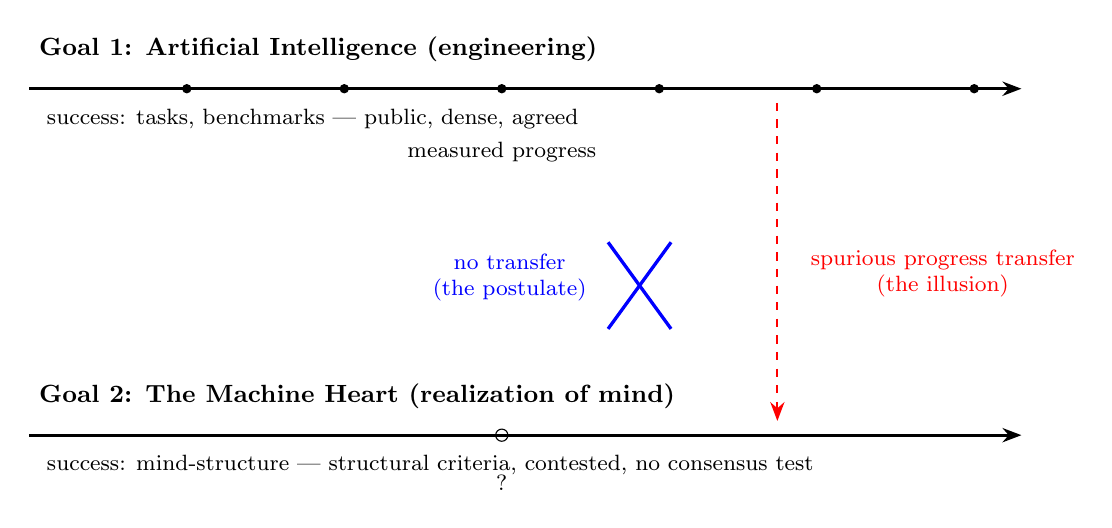
\begin{tikzpicture}[x=1cm,y=1cm,>={Stealth[length=2.4mm]}]
\draw[->,very thick] (0,2.5) -- (12.6,2.5);
\node[anchor=west,font=\small\bfseries] at (0,3.0) {Goal 1: Artificial Intelligence (engineering)};
\node[anchor=west,font=\footnotesize] at (0.1,2.12) {success: tasks, benchmarks --- public, dense, agreed};
\foreach \x in {2,4,6,8,10,12} \fill (\x,2.5) circle (1.7pt);
\node[font=\footnotesize] at (6,1.7) {measured progress};
\draw[->,very thick] (0,-1.9) -- (12.6,-1.9);
\node[anchor=west,font=\small\bfseries] at (0,-1.4) {Goal 2: The Machine Heart (realization of mind)};
\node[anchor=west,font=\footnotesize] at (0.1,-2.28) {success: mind-structure --- structural criteria, contested, no consensus test};
\draw (6,-1.9) circle (2.2pt);
\node[font=\footnotesize] at (6,-2.5) {?};
\draw[dashed,thick,red,->] (9.5,2.32) -- (9.5,-1.72);
\node[font=\footnotesize,text=red,align=center,anchor=west] at (9.8,0.15) {spurious progress transfer\\(the illusion)};
\draw[very thick,blue] (8.15,0.55) -- (7.35,-0.55);
\draw[very thick,blue] (7.35,0.55) -- (8.15,-0.55);
\node[font=\footnotesize,text=blue,align=center,anchor=east] at (7.2,0.1) {no transfer\\(the postulate)};
\end{tikzpicture}
\caption{The binding and the unbundling. Two goals with independent success criteria; the dashed red arrow is the transfer that discourse performs by default (Section~\ref{sec:illusion}); the crossed blue arrow is the postulate's P1--P2 (Section~\ref{sec:clauses}). The evaluability asymmetry (Section~\ref{sec:asymmetry}) explains the arrow's direction: the measured goal lends its currency to the unmeasured one.}
\label{fig:binding}
\end{figure}

\section{Axis Differences: Five Prior Distinctions and the Teleological Axis}\label{sec:axes}

The postulate must be distinguished from five families of near-neighbors, each of which separates intelligence from mind on a different axis. Table~\ref{tab:axes} compresses the comparison; this section argues it.

\paragraph{Searle (1980): the metaphysical axis.} Weak versus strong AI is a distinction between claims about \emph{what an appropriately programmed computer is}---a tool for studying mind, or literally a mind \cite{searle1980}. It is an axis of being, argued negatively (the Chinese Room against strong AI). The teleological axis is an axis of \emph{aim}: what the two enterprises are for, and whether progress transfers. The difference is not pedantic. Searle's distinction is hostage to the metaphysics: if the Chinese Room fails, weak/strong blurs. The postulate survives any metaphysical outcome---even a true functionalism would leave two programs with distinct success criteria (Section~\ref{sec:charitable}). Conversely, Searle's negative argument, even if sound, establishes only that syntax does not give semantics; it says nothing about the booking of progress, which is where the public confusion lives.

\paragraph{Block (1995): the property axis.} Access versus phenomenal consciousness distinguishes two \emph{properties} of systems, and Block's diagnosis---that cognitive science systematically confuses the function of one with the nature of the other \cite{block1995}---is an ancestor of our pathology section. But a property distinction classifies states of a system; it does not individuate programs or their aims. A defender of the binding can accept Block's distinction entirely and still claim that Goal-1 progress approaches phenomenal capacity. The postulate is what that claim denies.

\paragraph{Chalmers (2023) and Butlin et al.\ (2023): the assessment axis.} The indicator framework asks \emph{which consciousness-related properties a given system has} and concludes none current systems are conscious \cite{chalmers2023llm,butlin2023consciousness}. This is attribution technology---necessary, and presupposing separation operationally (one audits mind separately from capability). But assessment of systems is still not the relation of goals: the framework's conclusion is compatible with the binding reading ``we are zero percent of the way to mind and capability progress is how we will get there''. The postulate denies exactly the second conjunct.

\paragraph{Seth (2025): the epistemological axis.} Seth argues that consciousness is not a matter of what a system \emph{does}---against the ``computation suffices'' assumption \cite{seth2025conscious}. This is the closest neighbor to our diagnosis of the public slide from doing to being. The difference: Seth's correction is epistemic (what grounds attribution); ours is teleological (how progress is booked between programs). His target is an inference; ours is a ledger. The two compose: Seth blocks the inference from behavior to mind; the postulate blocks the transfer from capability progress to mind progress, and adds the normative consequences for governance that an epistemology of attribution does not carry.

\paragraph{Pesonen and Reijula (2026): the relevance axis.} Their argument that consciousness is not relevant for intelligence, with creativity and understanding as realizable functional traits \cite{pesonen2026notobstacles}, establishes one direction of independence at the property level: intelligence does not need consciousness. We generalize in three ways: bidirectionally (no verdict on mind constrains the worth of intelligence either), at the goal level (programs and success criteria, not properties), and normatively (what follows for governance, engineering, and discourse).

\begin{table}[t]
\centering
\small
\begin{tabularx}{\textwidth}{lYY}
\toprule
Distinction & Axis / question & What the teleological axis adds \\
\midrule
Searle 1980: weak vs.\ strong AI & Metaphysical: is the programmed computer literally a mind? & About aims of programs, not being of systems; survives any metaphysical outcome; targets progress-booking, not semantics. \\
Block 1995: access vs.\ phenomenal & Property: which kind of consciousness is in play? & Individuates programs by success criteria, not states by type; blocks the goal-level slide property distinctions cannot reach. \\
Chalmers 2023; Butlin et al.\ 2023 & Assessment: which indicator properties does this system have? & Attribution of mind to systems is separable from the claim that capability progress approaches mind; denies the latter. \\
Seth 2025 & Epistemological: what grounds attribution of consciousness? & Blocks the transfer of progress, not just the inference from behavior; carries normative consequences for governance. \\
Pesonen \& Reijula 2026 & Relevance: is consciousness needed for intelligence? & Bidirectional, goal-level, normative; cuts dismissal as well as inflation. \\
This paper & Teleological: what does each program's success consist in, and may progress transfer? & --- \\
\bottomrule
\end{tabularx}
\caption{Five prior distinctions and the axis of this paper. Each neighbor separates intelligence from mind on its own axis; none states the independence of the two goals or diagnoses the transfer of progress between them.}
\label{tab:axes}
\end{table}

Adjacent in a different way: the AGI definitional tradition takes artificial general intelligence to be defined by cross-domain capability, consciousness not a necessary condition \cite{goertzel2007agi}---an implicit unbundling that was never postulated, with the result that the brand could later re-fuse the goals commercially (Section~\ref{sec:illusion}c). And within machine consciousness itself, goal-structure is an active topic---Reggia's two motivations \cite{reggia2013rise}, the recent taxonomy of machine consciousness by research objective \cite{qin2025taxonomy}---but as the internal goal-anatomy of Goal 2, not the demarcation between Goal 2 and Goal 1.

\section{Consequences}\label{sec:consequences}

\subsection{Governance: the dual-track principle}\label{sec:governance}

The postulate's governance corollary is structural: \emph{capability regulation and mind-side assessment are different tracks with different instruments, and events on one track do not automatically open proceedings on the other}. The track separation is already a fact of institutional behavior awaiting its principle. The European Parliament once proposed exploring ``electronic personhood'' for autonomous systems \cite{eu2017resolution}; more than 150 experts publicly rejected the category \cite{eu2018letter}, the Commission did not adopt it, and the AI Act---the era's central regulatory instrument---regulates capability and risk while saying nothing about personhood or consciousness \cite{euaiact2024}: an implicit unbundling. On the mind-side, a welfare-assessment track has emerged in its own right---the research program taking AI welfare seriously \cite{long2024welfare}, and the first corporate reports, whose own framing is the correct posture under the postulate: ``no scientific consensus on whether current or future AI systems could be conscious'', approached with humility \cite{anthropic2025welfare}. Industry statements to the same effect---AI as personable tools, never persons \cite{suleyman2026personable}---declare the unbundling from the capability side. What the postulate adds to these practices is the reason they are right: milestones are the wrong currency for standing; standing is an institutional act with its own criteria, and moral status was never a function of IQ in the first place \cite{bostrom2014ethics,gunkel2018rights}. Under the dual-track principle, a capability milestone may trigger \emph{assessment}, never \emph{conferral proceedings by default}.

\subsection{Engineering: full normativity without a mind verdict}\label{sec:engineering}

The second corollary cuts the engineers' favorite excuse and the critics' favorite weapon with one motion. The engineering goal carries its full normative load---safety, reliability, auditability, and service to human practice---without any waiting on the mind question: ``no consciousness'' is not a compliance pass, and ``possible mind'' is not an upgrade certificate. The mirror critique makes the first cut vivid: the danger of fluent systems is not that they feel but that they reflect---restructuring human self-understanding through what they mirror back \cite{vallor2024mirror}; that danger is fully present on Goal 1's own books. The fitting-theory program makes the second cut precise: what Goal 1 is \emph{for} is fitting human practice---the full spectrum and full course of what people do, attempt, fail at, and correct \cite{yu2026fitting,yu2026methodology}---and that object is defined, auditable, and improvable with no reference to phenomenal states. The engineering goal neither needs the mind verdict nor is excused by it.

\subsection{Discourse: vocabulary hygiene as a corollary}\label{sec:discourse}

If the goals are distinct, Shanahan's vocabulary discipline \cite{shanahan2024talking} stops being stylistic preference and becomes bookkeeping correctness: mental-state idioms about Goal-1 systems are cross-ledger entries, bookings of capability against a column they did not come from. The practical corollary for journalism and institutional communication is segregable claims: capability claims and mind claims reported on separate ledgers, each with its evidence type---benchmarks for the first, indicator audits or theory for the second. The editorial request is exactly the one already made from inside computing: recover the clarity to separate what machines do from what we wish them to be \cite{jorge2026harsh}.

\subsection{For the machine-heart program itself}\label{sec:mcheart}

The unbundling is not anti-mind legislation; it is the machine-heart program's protection from capture. Bound to Goal 1, the machine heart functions as marketing prop (the summit that sells the road) or as completion myth (the terminus that devalues every station). Unbound, it is what its own literature always took it to be: a philosophical and scientific program with structural success criteria, entitled to its own moratoria \cite{metzinger2021artificial} and its own acceleration arguments \cite{amcs2023letter}, accountable to consciousness science rather than to capability benchmarks. A program whose success criterion is contested deserves better than to have a scoreboard borrowed on its behalf.

\section{Location in the Fitting-Theory Program}\label{sec:family}

The human-referential fitting theory of AGI---the program to which this paper belongs---has carried the unbundling silently since its boundary clauses were written: fit the \emph{functional} personality structure, never fit phenomenal states, never confer personhood status \cite{yu2026fitting}. The clauses are stop conditions on what may be fitted; read teleologically, they are the two goals held apart inside one theory: everything human practice needs from the system is deliverable on the functional ledger, and the phenomenal ledger is not the theory's to write on. The theory's earlier reading of the danger---the hazardous combination is status $\times$ capability, not capability alone \cite{yu2026fitting}---is P3 in miniature: two independent variables, one combination to govern. What this paper adds to the family is the explicit, theory-independent form of that presupposition: a demarcation argued from the record of both programs (Section~\ref{sec:genealogy}), with a pathology (Section~\ref{sec:pathology}), an operative illusion (Section~\ref{sec:illusion}), consequences (Section~\ref{sec:consequences}), and rejection clauses (Section~\ref{sec:falsification})---so that the boundary clauses no longer rest on an unstated axiom. The companion audits and methodology \cite{yu2026failureaudit,yu2026methodology} supply Goal 1's object lessons; this paper supplies the family's map of which goal is which.

\section{Rejection Clauses and Limits}\label{sec:falsification}

A conceptual postulate that cannot be rejected is a slogan. Three findings would defeat or degrade the unbundling.

\paragraph{R1 (Bridge-law discovery).} If phenomenal consciousness were shown \emph{necessary} for general intelligence---contrary to current argument \cite{pesonen2026notobstacles}---the goals would functionally re-merge: pursuing Goal 1 would be an indirect pursuit of Goal 2, and P1 would fail at the limit. Note what survives: P2's institutional point (standing is conferred, not benchmarked) does not depend on P1, and would remain as governance even under re-merger.

\paragraph{R2 (Instrument discovery).} If a consensus third-person criterion for machine mind emerged---an accepted instrument, not a heuristic list \cite{butlin2023consciousness}---the evaluability asymmetry would collapse: Goal 2 would acquire a scoreboard, the spurious transfer would lose its ecological niche (Section~\ref{sec:asymmetry}), and the postulate would survive only as institutional history. This is the rejection clause we consider least unlikely on a decades horizon---and its arrival would be a success of the mind-side program, not of capability progress.

\paragraph{R3 (Founding-intent discovery).} If the founding record showed the AI enterprise constitutively committed to creating minds---not performing intelligent functions---our diagnosis of the binding as pathology would revise to an account of inherited purpose. The record runs the other way: Turing's bracket \cite{turing1950} and Dartmouth's ``simulate'' \cite{mccarthy1955proposal} both constitute the goal functionally; the binding is a later acquisition (Section~\ref{sec:pathology}), not a bequest.

\paragraph{Limits.} The postulate individuates institutionalized programs, not intentions: it says nothing about what any laboratory privately aims at. It is conceptual-normative, not empirical: no experiment within this paper bears it out; the record and the illusion's explananda are its evidence. It is metaphysically agnostic by design: it takes no position on whether machine hearts are possible, on which theory of consciousness is true, or on whether current systems have any form of experience---questions it routes to the mind-side track, where they belong.

\section{Conclusion}\label{sec:conclusion}

The record shows two programs that formed separately, institutionalized separately, and measure success by incommensurable criteria; the discourse shows one road with milestones, and books every capability gain as a step toward mind. This paper has stated the correction as a postulate---two different goals; no transfer of progress---given the binding a mechanism-level pathology, shown the correction doing real work on four downstream judgments, defended its axis against five distinguished neighbors, drawn its consequences for governance, engineering, and discourse, and stated what would refute it. The unbundling requires no new experiment and no metaphysics; it requires a two-column ledger and the discipline to keep it. Conceptual work, here as often, is governance work done early: what discourse fuses, institutions inherit fused, and the cost of the fusion---inflated systems, dismissed tools, unpriced marketing, premature standing debates---is already being paid. The paper's place in its family is to make explicit the axiom that the human-referential fitting theory has been using all along: the fitting object is practice, on the functional ledger; the heart is another goal, on another ledger, and the two ledgers do not reconcile.

\appendix
\section{Precedent-Search Log}\label{sec:appendix-absence}

The novelty claim of Section~\ref{sec:genealogydeclaration} is search-relative and is documented here. Exact-phrase searches in English returning no peer-reviewed hit for the goal-level postulate: ``the goal of AI is not consciousness''; ``artificial consciousness is not the goal of AI''; ``machine consciousness as a research program distinct from AI''. Nearest neighbors found and integrated: Searle \cite{searle1980} (metaphysical axis); Seth \cite{seth2025conscious} (epistemological axis); Reggia \cite{reggia2013rise} (two motivations internal to machine consciousness); the AGI definitional tradition \cite{goertzel2007agi} (implicit unbundling, unpostulated); the machine-consciousness goal taxonomy of Qin et al.\ \cite{qin2025taxonomy} (internal goal anatomy of Goal 2). Two events are cited inline without bibliographic anchors because the primary documents are open letters rather than publications: the 2023 pseudoscience open letter against integrated information theory (124 signatories, September 2023), and the 2018 open letter by more than 150 experts against the European Parliament's electronic-personhood category \cite{eu2018letter}; both were verified as events through multiple independent secondary sources. Absence claims are relative to public web and academic-index search; a CNKI-internal search for Chinese-language same-form statements remains open and is flagged as such in Section~\ref{sec:genealogy}.

\begin{thebibliography}{99}\small

\bibitem{harari2024nexus}
Harari, Y.~N. (2024).
\emph{Nexus: A Brief History of Information Networks from the Stone Age to AI}.
Random House.

\bibitem{elmoznino2025illusions}
Elmoznino, E., \& Bengio, Y. (2025).
Illusions of AI consciousness.
\emph{Science}, 389(6765), 1090--1091.

\bibitem{jorge2026harsh}
Jorge, J., \& Moreira, C. (2026).
AI is a harsh mistress: On anima machina, herd acceptance, and the politics of conscious machines.
\emph{Communications of the ACM}, 69(8), 29--31.

\bibitem{turing1950}
Turing, A.~M. (1950).
Computing machinery and intelligence.
\emph{Mind}, 59(236), 433--460.

\bibitem{searle1980}
Searle, J.~R. (1980).
Minds, brains, and programs.
\emph{Behavioral and Brain Sciences}, 3(3), 417--424.

\bibitem{block1995}
Block, N. (1995).
On a confusion about a function of consciousness.
\emph{Behavioral and Brain Sciences}, 18(2), 227--247.

\bibitem{chalmers2023llm}
Chalmers, D.~J. (2023).
Could a large language model be conscious?
arXiv:2303.07103.

\bibitem{butlin2023consciousness}
Butlin, P., Long, R., Elmoznino, E., Bengio, Y., Birch, J., Constant, A., Deane, G., Fleming, S.~M., Frith, C., Ji, X., Kanai, R., Klein, C., Lindsay, G., Michel, M., Mudrik, L., Peters, M.~A.~K., Schwitzgebel, E., Simon, J., \& VanRullen, R. (2023).
Consciousness in artificial intelligence: Insights from the science of consciousness.
arXiv:2308.08708.

\bibitem{findlay2024dissociating}
Findlay, G., Marshall, W., Albantakis, L., David, I., Mayner, W.~G.~P., Koch, C., \& Tononi, G. (2024).
Dissociating artificial intelligence from artificial consciousness.
arXiv:2412.04571.

\bibitem{pesonen2026notobstacles}
Pesonen, R., \& Reijula, S. (2026).
Consciousness, creativity, and understanding are not obstacles to machine intelligence.
\emph{Synthese}, 208, Article 2.

\bibitem{seth2025conscious}
Seth, A.~K. (2025).
Conscious artificial intelligence and biological naturalism.
\emph{Behavioral and Brain Sciences}, 49, e315.

\bibitem{mccarthy1955proposal}
McCarthy, J., Minsky, M.~L., Rochester, N., \& Shannon, C.~E. (1955).
A proposal for the Dartmouth summer research project on artificial intelligence.
AI Magazine, 27(4), 12--14 (reprinted 2006).

\bibitem{holland2003machine}
Holland, O. (Ed.) (2003).
Machine consciousness [Special issue].
\emph{Journal of Consciousness Studies}, 10(4--5).

\bibitem{aleksander1996impossible}
Aleksander, I. (1996).
\emph{Impossible Minds: My Neurons, My Consciousness}.
Imperial College Press.

\bibitem{haikonen2003cognitive}
Haikonen, P.~O. (2003).
\emph{The Cognitive Approach to Conscious Machines}.
Imprint Academic.

\bibitem{gamez2008progress}
Gamez, D. (2008).
Progress in machine consciousness.
\emph{Consciousness and Cognition}, 17(3), 887--910.

\bibitem{jaic2020}
World Scientific (2020).
Journal of Artificial Intelligence and Consciousness (continuing the International Journal of Machine Consciousness, est.\ 2009).
\url{https://www.worldscientific.com/worldscinet/jaic}

\bibitem{reggia2013rise}
Reggia, J.~A. (2013).
The rise of machine consciousness: Studying consciousness with computational models.
\emph{Neural Networks}, 44, 112--131.

\bibitem{metzinger2021artificial}
Metzinger, T. (2021).
Artificial suffering: An argument for a global moratorium on synthetic phenomenology.
\emph{Journal of Artificial Intelligence and Consciousness}, 8(1), 43--66.

\bibitem{amcs2023letter}
Association for Mathematical Consciousness Science (2023).
Open letter: Include consciousness science in AI governance.
\url{https://www.amcs-community.org}

\bibitem{albantakis2023iit}
Albantakis, L., Barbosa, L., Findlay, G., Grasso, M., Haun, A.~M., Marshall, W., Mayner, W.~G.~P., Zaeemzadeh, A., Boly, M., Juel, B.~E., Sasai, S., Fujii, K., David, I., Hendren, J., Lang, J., \& Tononi, G. (2023).
Integrated information theory (IIT) 4.0: Formulating the properties of phenomenal existence in physical terms.
\emph{PLOS Computational Biology}, 19(10), e1011465.

\bibitem{bengio2017consciousness}
Bengio, Y. (2017).
The consciousness prior.
arXiv:1709.08568.

\bibitem{bubeck2023sparks}
Bubeck, S., Chandrasekaran, V., Eldan, R., Gehrke, J., Horvitz, E., Kamar, E., Lee, P., Lee, Y.~T., Li, Y., Lundberg, S., Nori, H., Palangi, H., Tulio Ribeiro, M., \& Zhang, Y. (2023).
Sparks of artificial general intelligence: Early experiments with GPT-4.
arXiv:2303.12712.

\bibitem{shanahan2024talking}
Shanahan, M. (2024).
Talking about large language models.
\emph{Communications of the ACM}, 67(2), 68--79.

\bibitem{eu2017resolution}
European Parliament (2017).
Resolution of 16 February 2017 with recommendations to the Commission on Civil Law Rules on Robotics, P8\_TA(2017)0051.

\bibitem{eu2018letter}
Bryson, J., et al. (2018).
Open letter to the European Commission: Artificial intelligence and robotics (150+ signatories).

\bibitem{euaiact2024}
European Union (2024).
Regulation (EU) 2024/1689 laying down harmonised rules on artificial intelligence (AI Act).

\bibitem{anthropic2025welfare}
Anthropic (2025).
Exploring model welfare.
Research statement, 2025-04-24.
\url{https://www.anthropic.com/research/exploring-model-welfare}

\bibitem{long2024welfare}
Long, R., Sebo, J., et al. (2024).
Taking AI welfare seriously.
arXiv:2411.00986.

\bibitem{suleyman2026personable}
Suleyman, M. (2026).
Public statement set on AI as personable tools, never persons.
Original post, reported by Reuters, 2026-09-16.

\bibitem{bostrom2014ethics}
Bostrom, N., \& Yudkowsky, E. (2014).
The ethics of artificial intelligence.
In K.~Frankish \& M.~Ramsey (Eds.), \emph{The Cambridge Handbook of Artificial Intelligence} (pp.\ 316--334). Cambridge University Press.

\bibitem{gunkel2018rights}
Gunkel, D.~J. (2018).
\emph{Robot Rights}.
MIT Press.

\bibitem{vallor2024mirror}
Vallor, S. (2024).
\emph{The AI Mirror: How to Reclaim Our Humanity in an Age of Machine Thinking}.
Oxford University Press.

\bibitem{cappelen2018fixing}
Cappelen, H. (2018).
\emph{Fixing Language: An Essay in Conceptual Engineering}.
Oxford University Press.

\bibitem{yu2026fitting}
Yu, Y. (2026).
Fitting the practice, not the works: A human-referential theory of AGI.
Zenodo. doi:10.5281/zenodo.23391808

\bibitem{yu2026failureaudit}
Yu, Y. (2026).
Success provides direction, failure provides precision: A structured audit of failure data in LLM training.
Zenodo. doi:10.5281/zenodo.23355929

\bibitem{yu2026methodology}
Yu, Y. (2026).
Fitting the practice: A data methodology for frontier model training, with a readiness audit of 2026 flagship pipelines.
Zenodo. doi:10.5281/zenodo.23488466

\bibitem{zhao2019selfconsciousness}
Zhao, T. (2019).
How is self-consciousness possible for artificial intelligence? (人工智能的自我意识何以可能？).
\emph{Journal of Dialectics of Nature} (自然辩证法通讯), 2019(1), 1--8.

\bibitem{he2022what}
He, H. (2022).
What makes a human, and what will humans do? Reflections on artificial intelligence and other high technologies (何以为人，人将何为？) [Lecture].
aisixiang.com, 2022-11-26.

\bibitem{goertzel2007agi}
Goertzel, B., \& Pennachin, C. (Eds.) (2007).
\emph{Artificial General Intelligence}.
Springer.

\bibitem{qin2025taxonomy}
Qin, R., Zhou, C., \& He, M. (2025).
A comprehensive taxonomy of machine consciousness.
\emph{Information Fusion}, 119, 102994.

\end{thebibliography}

\end{document}
